\documentclass[a4paper]{article}

\usepackage{fullpage}
\usepackage{natbib}
\usepackage{graphics}
\usepackage{multirow}
\usepackage[table]{xcolor}
\usepackage{graphicx}

\title{Automatic Assessment and Stenting of Arterial Stenosis}
\author{Concours CNRS 2012 -- Projet de Recherche}
\date{R\^omulo TEIXEIRA DE ABREU PINHO}

\begin{document}

\maketitle

\begin{noindent}
{\em Obs: I am a Brazilian native who has been living in France for two years. Despite my working knowledge of the French language, I am writing this project proposal in English, for efficiency reasons.}
\end{noindent}

\begin{abstract}
\hrule
\medskip
Atherosclerosis figures as one of the leading cardiovascular diseases, which remain as the major cause of death in developed countries. Image analysis and processing is an important tool in the diagnosis and treatment of vascular diseases. Minimally invasive interventions are increasingly becoming the treatment option of choice, given the reduced surgical risk for the patient. A good example is the use of stents to reopen arterial stenosis or to protect the dilated walls of aneurysms from further expansion. Stent choice remains, nevertheless, a subjective decision. An inadequate stent may migrate to another location, may exert exaggerated pressure on the arterial walls, may not properly cover the affected area, etc. This document describes a project proposal for the automatic detection and quantification of stenosis and aneurysms and for the automatic prediction of optimal patient-specific stent parameters. The proposed methods build upon the work presented in my PhD thesis, which focussed on the assessment and stenting of tracheal stenosis. They also integrate physical properties of arteries and stents, as well as stent deployment and blood flow simulations, into the stent choice process. 
\medskip
\hrule
\end{abstract}


\tableofcontents

\pagebreak

\hrule
\section{Context}
\hrule

\medskip
\medskip

Atherosclerosis figures as one of the leading cardiovascular diseases, which remain as the major cause of death in developed countries. Concomitantly, the use of images plays a very important role in the diagnosis, treatment, and follow up of vascular diseases. Likewise, minimally invasive interventions are becoming more available and are the preferred treatment option given the reduced surgical risk to the patient. The treatment of atherosclerosis (stenosis and aneurysms) using stents is a very good example that profits from both the use of images and minimally invasive interventions. 

A large variety of stents is available in the market. However, choosing the correct stent parameters (type, length, diameter, and deployment location) is challenging and remains a specialist-dependent and subjective task, which is mostly based on the expertise of the physician in charge. This problem attracts large attention and an event to compare the results of existing algorithms to aid in the detection and quantification of coronary stenoses will soon be organized (http://coronary.bigr.nl/stenoses).

In my PhD thesis, I showed that the choice of stents for the treatment of tracheal stenosis can be automated and simplified with the use of statistical shape models. The proposed method solves the problem of automatically determining the location of the stricture, its length, and the degree of narrowing by giving an estimation of the patient's healthy trachea, that is, if stenosis were not present. From this estimation, followed by a segmentation of the narrowed trachea, determining the parameters of the stenosis and consequently of the patient-specific stent is straightforward. 

Despite being a natural extension of my thesis, applying the method proposed for the trachea to the case of arterial stenosis and aneurysm is far from trivial. Many challenges exist, first and foremost the automatic segmentation and labelling of the arterial tree, which remains an open problem. Additionally, in order to optimize the stent choice, several parameters need to be taken into account, such as the physical properties of the arterial wall and of the stents themselves and the estimation of the blood flow after deploying the stent. 

I intend to study and solve these problems and to apply the solutions in the clinical domain. In order to achieve it, I would like to be part of the {\it Centre de Recherche Et d�Applications en Traitement de l�Image et du Signal} (CREATIS), whose expertise in the domain of segmentation of images of the vascular system and the use of stents in the treatment of arterial stenoses and aneurysms will be an invaluable contribution to the project.

\medskip
\medskip

\hrule
\section{Project Description}
\hrule

\medskip
\medskip

The objective of the proposed project is to develop a solution for the problem of automatic stent choice in the treatment of vascular stenoses and aneurysms. To date, such problem has only been solved with semi-automatic methods, with a very subjective aspect, which is the determination of the healthy arterial diameter and the extension of the stenosis or the aneurysm. My goal is to improve this solution with an automatic process that optimizes the choice of stent type, length and diameter. In the following, I present the main challenges involved in the project and how I intend to solve them. 

\subsection{Estimation of Healthy Arteries}

In my PhD thesis, I proposed a method for the estimation of healthy tracheae from CT images of patients suffering from tracheal stenosis. This method is based on the construction of a statistical model \citep{Cootes} of 3D surfaces of healthy tracheae. When the model is registered to a CT scan of a patient with tracheal stenosis, it is capable of matching the parts of the tracheal wall that are healthy while at the same time estimating the shape of the remaining parts as if they were healthy. This method showed very promising results \citep{Pinho:Trachea4}.

A natural extension of my thesis is the application of the proposed method in the cardiovascular domain. Since arteries, as well as tracheae, are objects of tubular topology, and the characteristics of their stenoses are roughly the same, it is intuitive to believe that the method will also be able to estimate the shape of healthy arteries from images of patients with arterial stenosis. This rule also tends to apply in the case of aneurysms, as long as there are enough healthy regions around the location of the swelling.

I will adapt the method I proposed for tracheal stenosis so that it can be used with narrowed and swelled arteries. I believe that in the first instance, the method developed for the trachea can be used as is. I will build a training set of healthy artery sections using segmentation methods available in the literature, for example \citep{Florez2}. In this way, the problem is reduced to modelling objects of tubular shape, without bifurcations, resembling the case of the trachea. Since healthy artery sections tend to appear with good contrast in the images, their segmentation is in principle a relatively straightforward task. 

The main difficulty lies in the segmentation of the arterial tree and the corresponding surface representation to be used in the statistical model. To the best of my knowledge, statistical shape models of tree-like structures have not been proposed yet. In the next phase of the project, I intend to employ existing surface representation methods \citep{Florez, Antiga} and benefit from its branch nomenclature in order to establish correspondences between the shapes of the statistical model's training set, which is an important step in the model construction. 

\subsection{Segmentation of the Arterial Tree}

The segmentation of the arterial tree has been a topic of study for quite some time, but the automatic segmentation remains an open problem \citep{ORKI-08}. In the context of this project, the segmentation task is subdivided into two objectives: 1) the segmentation of healthy arteries; 2) segmentation of arteries with stenosis. Each is detailed in the following sections.

\subsubsection{Healthy Arteries}

This segmentation problem has much in common with the segmentation of airway tree, for which I also proposed an automatic solution in my PhD thesis, with interesting results \citep{Pinho:Airways2}. The method uses an iterative region growing algorithm with adaptive, cylindrical ROI's that simplifies the detection and elimination of leaks, a common problem in region growing. The method also includes an initialization step to automatically detect the starting point of the trachea, which is given as a seed point to the region growing algorithm (Figure \ref{fig:airways}). 

\begin{figure}%
\centering
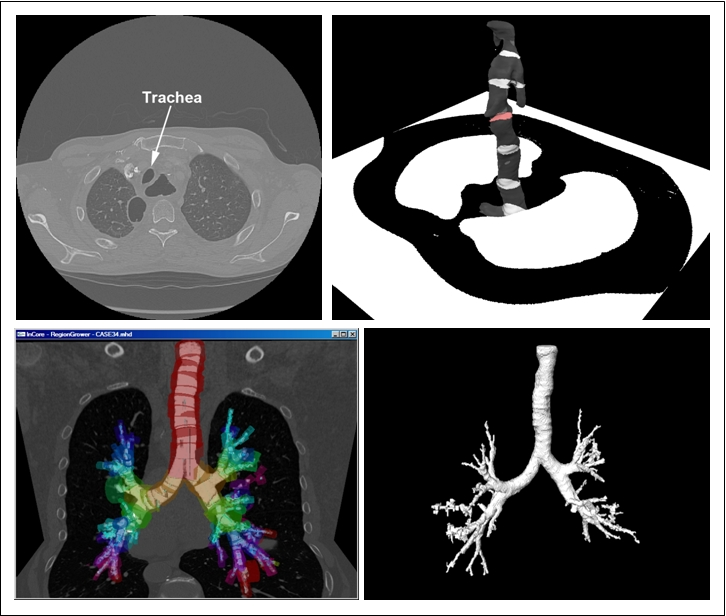
\includegraphics[width=0.5\columnwidth]{research_interests_airways.jpg}%
\caption{Segmentation of the airway tree as proposed in \citep{Pinho:Airways2}.}%
\label{fig:airways}%
\end{figure}

My intention is to apply this method to the segmentation of healthy arteries and to compare it with other segmentation methods \citep{Florez2, Antiga}. A challenge in this case will be the detection of a starting point for the segmentation. Tube enhancement filters \citep{ORLO-09} may help in at least isolating the tubular structures in the image, from where  the detection process may be triggered. 

\subsubsection{Narrowed Arteries}
\label{sec:narrowedarteries}

The segmentation of the healthy arterial tree is an important step in the construction of the statistical shape model. But similarly to tracheal stenoses, segmenting the narrowed arteries is an important step in the automatic calculation of parameters of the stricture. My experience with the segmentation of the trachea, however, has demonstrated that the segmentation of narrowed tube-like structures in medical images may be difficult. Region growing, for example, tends to fail to recover the correct tube wall if the narrowing is too severe and the lumen is not completely visible in the image. In my thesis, I used the estimation of the healthy trachea as initialization of the a deformable model to segment the narrowed tube. The proposed deformable model, based on the snake model proposed by \cite{Kass}, was able to correctly segment the tracheal wall even in the more difficult cases. Still, noise and the presence of neighbouring organs may hinder the segmentation process, and user intervention may still be necessary \citep{Pinho:Trachea7}.

I will thus experiment with the deformable model I proposed in my thesis in order to automatically segment narrowed arteries. The idea will still be to initialize the model with the estimation of the healthy artery obtained with the statistical shape model. I expect that this method will give better results then other solutions in the literature \citep{CARR-07,Florez2,Antiga,Bemmel}, but an in-depth comparison with those algorithms will be necessary.

\subsection{Stent Choice}

Physicians intuitively estimate the healthy shape of the narrowed artery when quantifying the stenosis or the aneurysm. With the approaches described above, I expect to be able to mimic the physician's work in a methodological and mathematical manner. After the estimation of the healthy artery shape, we are ready to automatically detect the exact location of the stenosis and to quantify it. For this, I will once again use the method I proposed in my PhD thesis \citep{Pinho:Trachea4}, which tracks changes in the cross-sectional area of the narrowed tube relative to the estimated healthy tube, but other similar approaches may be effective as well \citep{Florez2}.

Once the stenosis or aneurysm has been detected and quantified, the parameters of the stent are trivially obtained. At this point, the whole chain of the proposed project will be finished. However, the effectiveness of the predicted stent can only be verified after it has been deployed in the patient's artery. If the stent is inadequate, it may migrate to another location or strain the arterial wall. 

For this reason, I will add to the stent prediction parameters derived from the physical properties of the artery and of the stent itself. In addition, every predicted stent will be used in a blood flow simulation step such that its effectiveness can be further verified. From the simulations, other parameters will be extracted and added to the decision process. In this way, the proposed method will be turned into an optimization process on several variables. Some of them will impact the estimation of the artery's healthy shape, some will impact the stent choice.

\subsubsection{Extending the Statistical Shape Model}

When the statistical model of healthy arteries is registered to an image of a patient with atherosclerosis, the registration (as implemented in my PhD thesis) is an iterative, edge-based search. At each iteration, the new locations of the landmarks that describe the surface of the artery are determined and a least squares minimization process makes the shape generated by the statistical model fit to the new point locations. Since the model is constrained by the (healthy) shape information contained in it, the resulting surface will resemble a healthy artery.

A ``healthy artery'' in this context means that only the geometrical variation about the arteries is captured by the statistical model. Still, arteries have physical properties such as elasticity, malleability, and bending, that are not explicitly encoded in the model. At the best, the geometric information may implicitly contain some aspects of the referred properties. 

I will then study the physical properties of arteries in order to add such information to the shape model. As a result, when registering the model to the patient's image these properties will further constrain the deformation and I expect that they will help giving a better estimation of the healthy arterial shape. 

In the same way, I will further extend the model with the physical properties of the stents. Since the ultimate objective of the project is the prediction of stents, it is reasonable that their physical properties be an extra parameter in the construction of the statistical model. Consequently, when registering the model to the patient's image, not only will the properties of the artery play a role, but we will at the same time influence the estimation of the healthy artery with the properties of the stent. 

\subsubsection{Physically-based Segmentation of the Deformed Artery}

In the same way that the statistical shape model can be extended, so can be the segmentation of narrowed and swelled arteries. Originally, the snake model proposed by \citet{Kass} depends on internal and external energies to deform the surface (or contour) towards the desired image feature. The internal energies take only elasticity and bending into account. 

I will add extra energy terms with arteries' physical properties in order to restrict (or improve) the surface deformations, so that the model can better adapt to the arteries' boundaries. Such physical properties must also take into account those of narrowed and swelled regions, since the main object of this segmentation step is to correctly segment them.

\subsubsection{Simulations}

As stated previously, when the estimated healthy arterial shape and the segmented narrowed artery are obtained, the automatic detection and quantification of the stenosis or aneurysm tends to be trivial. The stent to be chosen, however, is the one that will optimize the blood flow after deployment. For this reason, new parameters can be added to the proposed model.

\paragraph{Stent Deployment}

\citet{Florez,deBeule} proposed methods for stent deployment simulations using deformable models and numerical methods. With these methods, it is possible to (visually) verify whether the predicted stent properly expands the narrowed region of the artery or whether it correctly bypasses the swelled region. 

My idea is to find a way to methodologically quantify these parameters, by using the stents' and arteries' physical properties, and to have measures for, e.g., arterial wall straining, stenosis/aneurysm coverage, stent deformation, etc. These parameters can be further added to the statistical shape model to improve the healthy shape estimation. Consequently, the model registration will tend to yield a shape with the best characteristics in terms of the stent vs. wall interaction as well.

\paragraph{Blood Flow}

Blood flow simulations already play an important role in stent design \citep{deBeule}. They are also extensively used for flow assessment after stent deployment \citep{Vuk,Gori}. However, to the best of my knowledge, such simulations have not yet been integrated in the stent choice process. 

To achieve such integration, my plan is to define a function of the blood flow subject to the stent parameters (physical properties, deployment location, length, and diameter). This function will then be maximized, such that the chosen stent is the optimal one for a certain patient. This optimization process will thus influence the entire workflow, from the estimation of the healthy arterial shape, passing through the segmentation of the narrowed/swelled artery, to the detection and quantification of the stenosis/aneurysm, and the final prediction of the stent parameters. In fact, I imagine an algorithm that implements the workflow depicted in Figure \ref{fig:workflow}. 


\begin{figure}%
\centering
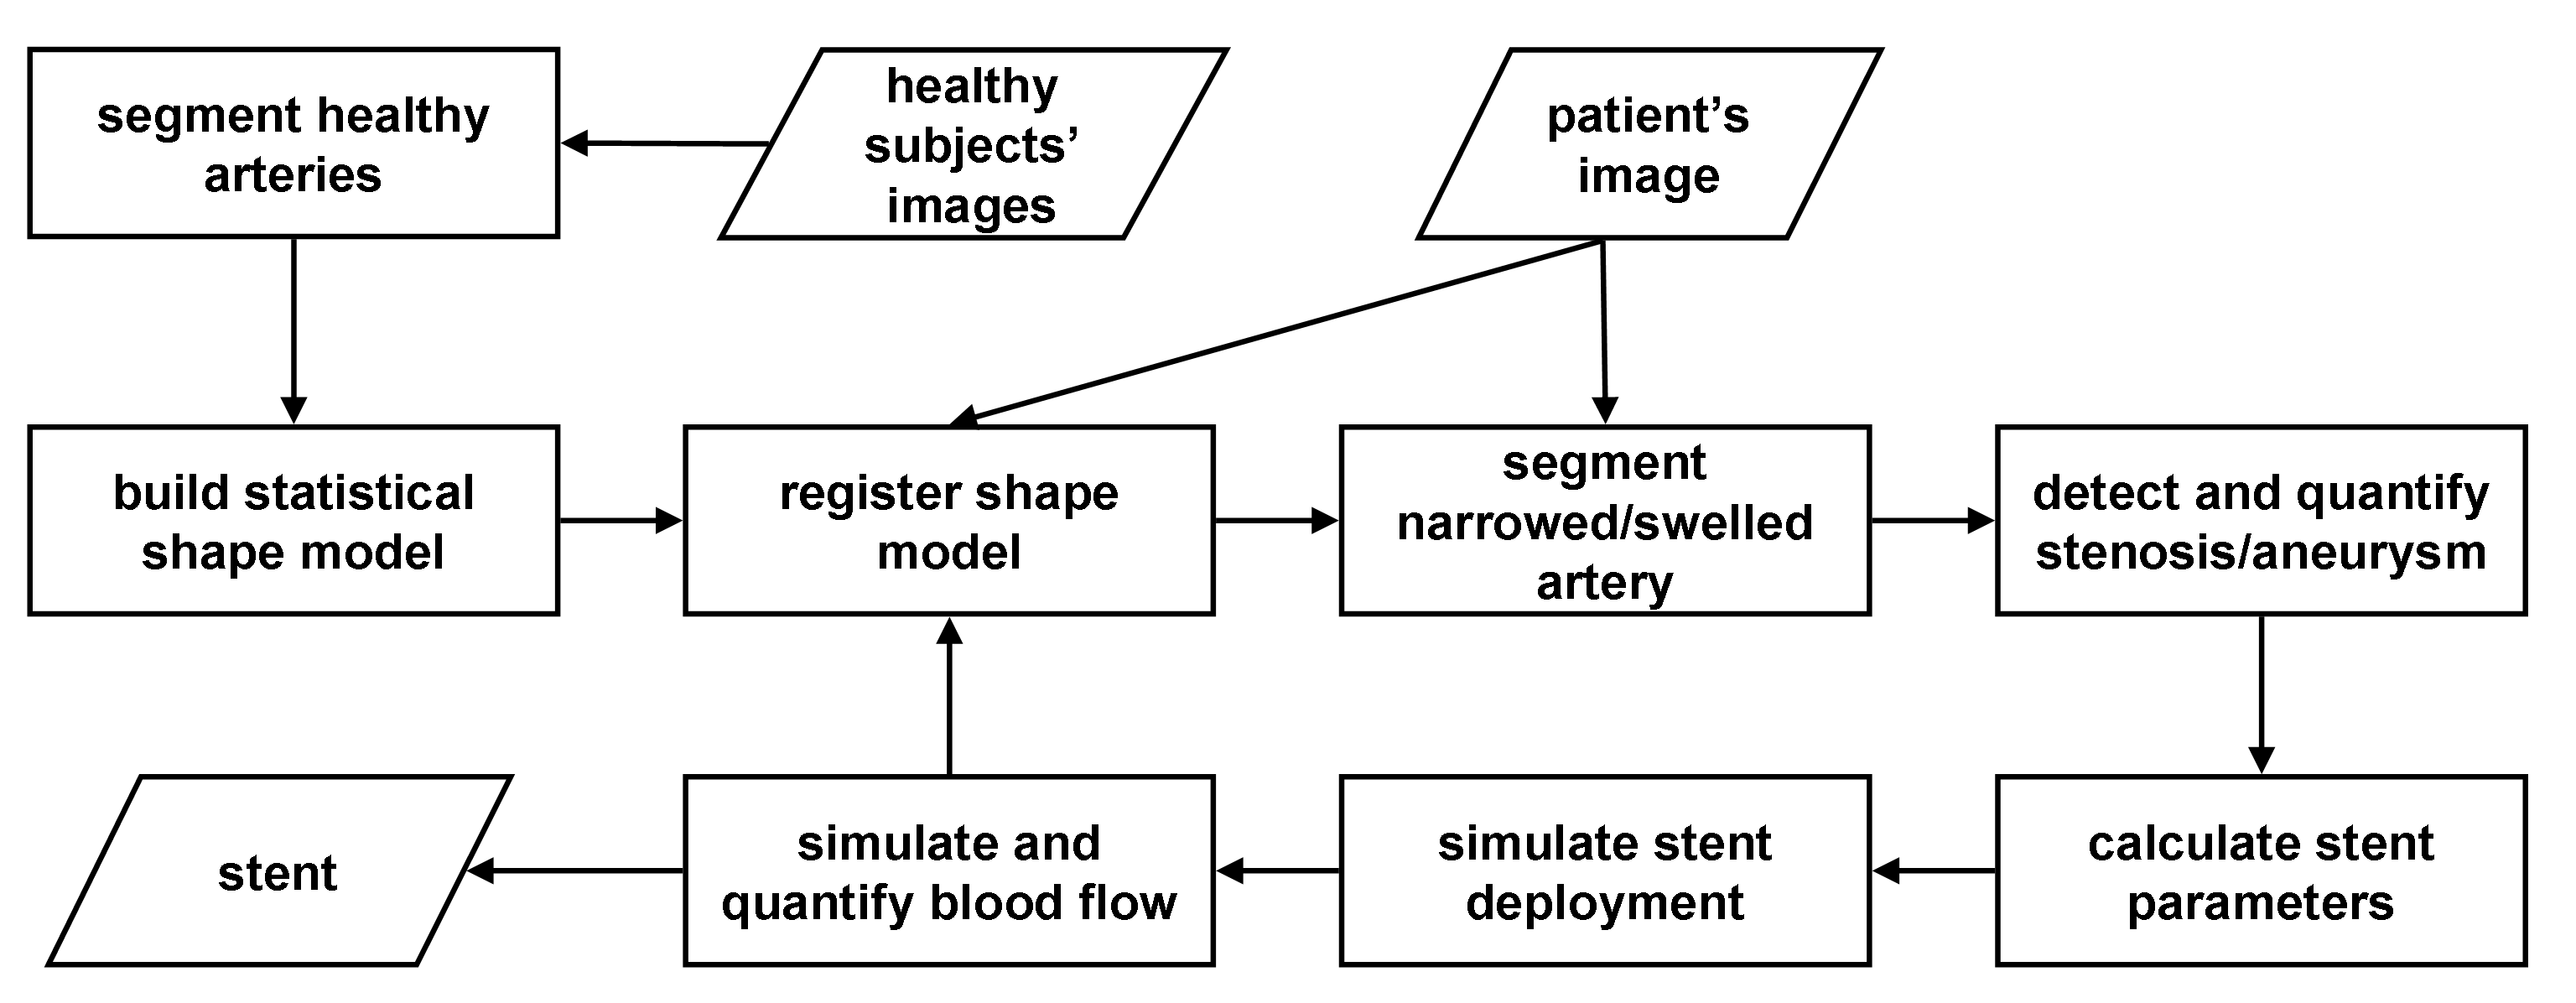
\includegraphics[width=0.8\columnwidth]{workflow.png}%
\caption{Workflow of the complete automatic stent prediction process.}%
\label{fig:workflow}%
\end{figure}

\subsection{GPU Acceleration}

In order to achieve the expected results with the proposed methods, a lot of computational power may be necessary. The blood simulations, for instance, require a large number of calculations. The proposed optimization process, as well, is a classic case study for the use of clusters and grids. I envision the use of such architectures, but bringing this computing power to the clinic is impractical and expensive. A more viable, yet powerful, solution is thus necessary.

The FASTRA technology is a successful attempt of building a desktop supercomputer using multiple GPU's. At the cost of a couple of high-end desktop computers, this technology yields computing power comparable to more than 256 CPU's working together, with proper GPU programming (http://fastra.ua.ac.be/en/index.html).

In GPU programming, however, memory transfers between the computer's main memory and the GPU may impose a severe bottleneck. Given the reduced memory size in graphics cards, relative to available RAM sizes, and the increasing size of medical image files, image buffers cannot be completely allocated in GPU memory. As a consequence, a smart memory transfer scheme must be devised. 

In my PhD thesis, I dealt with a similar problem, but in a different scale. Since image processing pipelines may require several simultaneous copies of the image buffer, current available RAM's may not be large enough. I therefore proposed an out-of-core solution for image processing based on sliding window cache and pre-fetching techniques. In other words, only the parts of the image that are necessary in a given moment reside in main memory. The other parts remain in disk. Using a-priori knowledge about the image traversal pattern of image processing algorithms, it is possible to predict which regions of the image will be needed in the future. These images can be asynchronously fetched from disk and stored in a cache before being requested by the algorithm. If the I/O operation is fast enough, it is very likely that the algorithm will not have to wait for the request complete \citep{Pinho:Cache1}. 

I believe that such an approach can similarly be applied in transfers between the computer's main memory and the GPU. I will then adapt the cache and pre-fetching method I proposed in my thesis and translate it to GPU-specific code. In this way, I expect that the stent choice optimization can be made without the need of the cluster structure.

\medskip
\medskip

\hrule
\section{Integration in the Laboratory, Collaborations, Schedule}
\hrule

\medskip
\medskip

\subsection{Laboratory}

My intention of joining the CREATIS group is on the one hand to benefit from their expertise in the several areas correlated to this project proposal. On the other hand, it will be my role to contribute to this expertise by bringing to the lab my own experience with the assessment and stenting of tracheal stenosis and applying it to the cardiovascular domain.

CREATIS have at their disposal an internal computer cluster and also the computation power of the {\it Centre de Calcul de L'Institut National de Physique Nucl\'eaire et de Physique des Particules} (CC-IN2P3). These will be invaluable tools for the simulation parts of the proposed project. 

Most importantly, CREATIS also profit from a very multidisciplinary nature and strong links with the clinical practice, most notably that of the {\it h\^opital neuro-cardiologique des Hospices Civiles de Lyon} (HCL) and of the {\it Centre L\'eon B\'erard} (CLB). This will give me the opportunity to evaluate the results of the proposed project with real patient data and to have immediate feedback from physicians. 

\subsection{Collaborations}

During my PhD in Belgium, I established a very good relationship with Prof. Dr. Jan Sijbers, my thesis supervisor, in the VisionLab group of the University of Antwerp. The group has extensive experience with medical image segmentation problems and modelling of cylindrical objects, which could be interesting in the context of this project. In addition, this is the group where the FASTRA technology was developed and the group is always interested in new applications for it. I would like to bring the VisionLab and CREATIS together during the course of the proposed project, so that they can benefit from each other's work.

My stay in Belgium also allowed me to get acquainted with the work of the Stent Research Unit of the University of Ghent. Their work is focussed on the design of stents using numerical simulations, on which much of this project may be based. 

I also envision collaborations with the academic and industrial partners of the European Project THROMBUS, whose aim is to evaluate the efficacy of the use of stents in neurological aneurysms. These partners, among them CREATIS, combine expertise in different areas and will certainly be a good source of information for my project.

Lastly, an opportunity will be open from early 2014, with the first calls for the UE project ``Horizon 2020''. This will probably be a good chance to join partners such as those in the THROMBUS project or establish new partnerships. 

\subsection{Tentative Schedule}

\begin{table}[h]\centering
\begin{tabular}{c|c|c|c|c|c|c|c|c|}
\cline{2-9}
 & \multicolumn{2}{|c|}{Y1} & \multicolumn{2}{|c|}{Y2} & \multicolumn{2}{|c|}{Y3} & \multicolumn{2}{|c|}{Y4} \\ \cline{2-9}
 & S1 & S2 & S3 & S4 & S5 & S6 & S7 & S8  \\ \hline
\multicolumn{1}{|c|}{Apply existing model} & \cellcolor{green} & & & & & & & \\ \hline
\multicolumn{1}{|c|}{Segmentation and modelling} & & \cellcolor{green} & \cellcolor{green} & \cellcolor{green} & & & & \\ \hline
\multicolumn{1}{|c|}{Stent choice and simulations} & & & & & \cellcolor{green} & \cellcolor{green} & \cellcolor{green} & \cellcolor{green} \\ \hline
\end{tabular}
\caption{Tentative project schedule for 4 years, subdivided into semesters.}
\label{tab:schedule}
\end{table}

Table \ref{tab:schedule} shows a tentative schedule for the proposed project. The objective in the short term, roughly the first 6 months, is to try to directly apply the statistical model I proposed in my thesis to cases of arterial stenosis and aneurysms. I have reasons to believe that this step tends to be rather straightforward, requiring only few modifications to the original method, if any. The possibly biggest challenge would be the segmentation and surface modelling of the arteries, which, in the first instance, could be simplified (e.g., not taking bifurcations into account) and accomplished with existing techniques so as to yield acceptable results in a short period of time. 

The following step, to be carried out during the next 18 months, will be the extension of the statistical model with anatomical information about the arterial tree. Bifurcations will also be taken into account. 

Finally, the remaining 24 months will be dedicated to the stent choice and simulation parts. The starting point of this step will be the stent choice with a generic stent and artery model. In other words, stents' and arteries' physical properties will not be taken into account. In this way, we will be able to at least evaluate if the generic stents computed with use of the statistical model are adequate. Later, blood flow and stent deployment simulation results will be used to improve the statistical model and, ultimately, the automatic stent choice.  

%\section{Conclusions}

\bibliographystyle{plainnat}
\bibliography{mybib,trachea,stents,artery}

\end{document}
